\chapter{Additional results}
This section contains the detailed studies on the expected results before the unblinding.
The goal of these studies is twofold, as they allow to gauge the expected performance
of the strategies, and to ensure the stability of the analysis by allowing a more in-depth investigation
on the uncertainties and their effect on the signal.

\section{Four lepton channel}
\label{sec:expected_4L}
The likelihood scans and the study on the impact of the systematic uncertainties for each of the strategies
in the four lepton channel are collected here.
First, the studies in the inclusive region are reported in Section~\ref{sec:expected_4L_inclusive}.
Then, the investigations for the triboson fiducial region are detailed in Section~\ref{sec:expected_4L_FSRcut}.

\subsection{Inclusive region}
\label{sec:expected_4L_inclusive}

\subsubsection{Likelihood scans}
% Likelihood scans with nuisance groups without the FSR cut
\label{sec:likelihood_scans_inclusive}
The extraction of the signal strength modifier $\mu$ proceeds through the maximisation of the likelihood,
as described in Section~\ref{sec:statistical_analysis}.
This procedure can be visualised by scanning the likelihood function for several values of the parameter $\mu$ while profiling the nuisance parameters.
For each value the best fit value of the nuisance parameters is computed,
and the resulting value of the likelihood is stored.
These points are then plotted as a function of $\mu$.

Usually the auxiliary quantity $-2\Delta\text{ln}\Likelihood$ (defined as $t_0$ in Equation~\ref{eq:test_statistic})
is used instead of the likelihood itself.
The width of the its profile is linked to the uncertainty on the estimate of $\mu$ from the fit.
More precisely, the set of values $\{ \mu / -2\Delta\text{ln}\Likelihood(\mu) < 1 (4) \}$ corresponds to the 68\usep\% (95\usep\%) confidence interval.

This procedure can also be performed by fixing the values of one or more nuisances instead of allowing them to be fitted by the algorithm.
The effect of fixing the value of one or more parameters is a reduction in the width of the likelihood shape.
This difference is ascribed to the effect of the frozen parameters.

Four groups of parameters are used in the following results:
\begin{itemize}
\item \textbf{theory:} uncertainties on the QCD scale, proton PDFs and on the value of \alpS;
\item \textbf{data-driven:} uncertainties related to the data-driven estimate of fake lepton or fake photon backgrounds;
\item \textbf{luminosity:} the uncertainty on the integrated luminosity corresponding to the data collected by the CMS experiment;
\item \textbf{others:} remaining experimental uncertainties, such as the lepton or photon efficiency scale factors or the \pileup weight;
\end{itemize}

\begin{figure}
  \centering
  \includegraphics[height=.33\textheight]{Figures/dataMC/Run2/phoCR/SR4P/SYS_mZZGloose_central_pow_\dataMCblind .pdf}
  \hfill
  \includegraphics[height=.33\textheight]{Figures/combine/inclusive/scan_\expobs_Run2_SR4P_phoCR_lepCR_mZZGloose.pdf}
  \caption{\captionScan{mass of the $\PZ\PZ\PGg$ system}{Loose}{cut-based ID}{d}{not }}
  \label{fig:scan_Run2_SR4P_phoCR_lepCR_mZZGloose}
\end{figure}

\begin{figure}
  \centering
  \includegraphics[height=.33\textheight]{Figures/dataMC/Run2/lepCR/SR4P/SYS_loosept_central_pow_\dataMCblind .pdf}
  \hfill
  \includegraphics[height=.33\textheight]{Figures/combine/inclusive/scan_\expobs_Run2_SR4P_phoMC_lepCR_mZZGloose.pdf}
  \caption{\captionScan{mass of the $\PZ\PZ\PGg$ system}{Loose}{cut-based ID}{s}{not }}
  \label{fig:scan_Run2_SR4P_phoMC_lepCR_mZZGloose}
\end{figure}

\begin{figure}
  \centering
  \includegraphics[height=0.33\textheight]{Figures/dataMC/Run2/lepCR/SR4P/SYS_mZZGwp90_central_pow_\dataMCblind .pdf}
  \hfill
  \includegraphics[height=.33\textheight]{Figures/combine/inclusive/scan_\expobs_Run2_SR4P_phoMC_lepCR_mZZGwp90.pdf}
  \caption{\captionScan{mass of the $\PZ\PZ\PGg$ system}{\texttt{wp90}}{MVA ID}{s}{not }}
  \label{fig:scan_Run2_SR4P_phoMC_lepCR_mZZGwp90}
\end{figure}

\begin{figure}
  \includegraphics[height=0.33\textheight]{Figures/dataMC/Run2/lepCR/SR4P/SYS_mZZGwp80_central_pow_\dataMCblind .pdf}
  \hfill
  \centering
  \includegraphics[height=.33\textheight]{Figures/combine/inclusive/scan_\expobs_Run2_SR4P_phoMC_lepCR_mZZGwp80.pdf}
  \caption{\captionScan{mass of the $\PZ\PZ\PGg$ system}{\texttt{wp80}}{MVA ID}{s}{not }}
  \label{fig:scan_Run2_SR4P_phoMC_lepCR_mZZGwp80}
\end{figure}

\begin{figure}
  \centering
  \includegraphics[height=.33\textheight]{Figures/dataMC/Run2/lepCR/SR4P/SYS_wp90pt_central_pow_\dataMCblind .pdf}
  \hfill
  \includegraphics[height=.33\textheight]{Figures/combine/inclusive/scan_\expobs_Run2_SR4P_phoMC_lepCR_wp90pt.pdf}
  \caption{\captionScan{transverse momentum of the photon}{\texttt{wp90}}{MVA ID}{s}{not }}
  \label{fig:scan_Run2_SR4P_phoMC_lepCR_wp90pt}
\end{figure}

\begin{figure}
  \centering
  \includegraphics[height=.33\textheight]{Figures/dataMC/Run2/lepCR/SR4P/SYS_MVAcut_central_pow_\dataMCblind .pdf}
  \hfill
  \includegraphics[height=.33\textheight]{Figures/combine/inclusive/scan_\expobs_Run2_SR4P_phoMC_lepCR_MVAcut.pdf}
  \caption{Likelihood scan for the signal strength parameter
    on the yield in the various bins of the photon MVA ID.
    \descriptionFakePhoton{s}.
    The FSR cut is not applied.
    The effect of groups of nuisance parameters on the uncertainty is assessed by sequentially fixing their value in the fit.
  }
  \label{fig:scan_Run2_SR4P_phoMC_lepCR_MVAcut}
\end{figure}

The uncertainty on the signal strength due to the statistics is between 0.35 and 0.50,
and is by far the largest contribution to the total.
This feature is observed for all of the strategies tested here.
The other groups of systematics have much lower impacts.
The theoretical uncertainties are around 0.03-0.05,
while the effect of the luminosity is around 0.03
and the rest of the experimental uncertainties amount to 0.06-0.08 of the signal strength.
The data-driven estimate, when split of the other experimental uncertainties,
adds an undertainty of 0.05-0.08 on the signal strength when estimating the fake photon background
with the data-driven method (Figure~\ref{fig:scan_Run2_SR4P_phoCR_lepCR_mZZGloose}).

\note{Temp}
The signal sample has a cross section of 22.02\usep{}fb, as reported in Table~\ref{tab:listofsamples}.
Assuming a signal strength of
$1.000^{+0.480}_{-0.406}$,
as extracted from
\todo{best strategy}, % TEMP MVAcut
the measured cross section for the production of $\Pp\Pp \to 4\Pl\PGg$ ($\Pl = \Pe,\,\PGm$) at a centre-of-mass energy of $13\TeV$ is
$22.02^{+10.57}_{-8.94}\usep\text{fb}$.


\subsubsection{Systematic impacts}
\label{sec:impacts_inclusive}
\providecommand{\impactswidthscale}{0.6}
The \nonprompt photon contribution is estimated using the data-driven approach.
The variable considered is $m_{\PZ\PZ\PGg}$.
The impacts of the systematic uncertainties on the expected results is shown in Figure \ref{fig:inclusive_cutID_phoCR_mZZGloose}.

\begin{figure}
  \centering
  \includegraphics[height=0.33\textheight]{Figures/dataMC/Run2/phoCR/SR4P/SYS_mZZGloose_central_pow.pdf}
  \hfill
  \includegraphics[height=0.33\textheight]{Run2_SR4P_phoCR_lepCR_mZZGloose_impacts.pdf}
  \caption{Distribution and impacts of the systematic uncertainties on the signal strength fit
    on the mass of the $\PZ\PZ\PGg$ system,
    using the Loose working point of the photon cut-based ID.
    The data-driven estimate for \nonprompt photons is used.
    The FSR cut is not applied.
  }
  \label{fig:inclusive_cutID_phoCR_mZZGloose}
\end{figure}

\begin{figure}
  \centering
  \includegraphics[height=0.33\textheight]{Figures/dataMC/Run2/lepCR/SR4P/lead_loose_pt_pow.pdf}
  \hfill
  \includegraphics[height=0.33\textheight]{Run2_SR4P_phoMC_lepCR_loosept_impacts.pdf}
  \caption{Distribution and impacts of the systematic uncertainties on the signal strength fit
    on the transverse momentum of the photon,
    using the Loose working point of the photon cut-based ID.
    \Nonprompt photons are estimated from simulation.
    The FSR cut is not applied.
  }
  \label{fig:inclusive_cutID_phoMC_loosept}
\end{figure}

\begin{figure}
  \centering
  \includegraphics[height=0.33\textheight]{Figures/dataMC/Run2/lepCR/SR4P/SYS_wp90pt_central_pow.pdf}
  \hfill
  \includegraphics[height=0.33\textheight]{Run2_SR4P_phoMC_lepCR_mZZGwp90_impacts.pdf}
  \caption{Distribution and impacts of the systematic uncertainties on the signal strength fit
    on the mass of the $\PZ\PZ\PGg$ system,
    using the \texttt{wp90} working point of the photon MVA ID.
    \Nonprompt photons are estimated from simulation.
    The FSR cut is not applied.
  }
  \label{fig:inclusive_mvaID_phoMC_mZZGwp90}
\end{figure}

\begin{figure}
  \centering
  \includegraphics[height=0.33\textheight]{Figures/dataMC/Run2/lepCR/SR4P/SYS_wp80pt_central_pow.pdf}
  \hfill
  \includegraphics[height=0.33\textheight]{Run2_SR4P_phoMC_lepCR_mZZGwp80_impacts.pdf}
  \caption{Distribution and impacts of the systematic uncertainties on the signal strength fit
    on the mass of the $\PZ\PZ\PGg$ system,
    using the \texttt{wp80} working point of the photon MVA ID.
    \Nonprompt photons are estimated from simulation.
    The FSR cut is not applied.
  }
  \label{fig:inclusive_mvaID_phoMC_mZZGwp80}
\end{figure}

\begin{figure}
  \centering
  \includegraphics[height=0.33\textheight]{Figures/dataMC/Run2/lepCR/SR4P/SYS_MVAcut_central_pow.pdf}
  \hfill
  \includegraphics[height=0.33\textheight]{Run2_SR4P_phoMC_lepCR_MVAcut_impacts.pdf}
  \caption{Distribution and impacts of the systematic uncertainties on the signal strength fit
    on the yield in the various bins of the photon MVA ID.
    \Nonprompt photons are estimated from simulation.
    The FSR cut is not applied.
  }
  \label{fig:inclusive_kin_phoMC_MVAcut}
\end{figure}


\subsection{Triboson fiducial region}
\label{sec:expected_4L_FSRcut}
The following results are derived after the application of the cut
designed to suppress FSR and enhance the fraction of events from triboson production diagrams,
described in Section~\ref{sec:FSR_cut}.
The target is the process $\Pp\Pp \to \PZ\PZ\PGg \to 4\Pl\PGg$.

\subsubsection{Likelihood scans}
\label{sec:likelihood_scans_FSRcut}

\begin{figure}
  \centering
  \includegraphics[height=.33\textheight]{Figures/dataMC_FSRcut/Run2/phoCR/SR4P/SYS_mZZGloose_central_pow\dataMCblind .pdf}
  \hfill
  \includegraphics[height=.33\textheight]{Figures/combine/FSRcut/scan_\expobs_Run2_SR4P_phoCR_lepCR_mZZGloose.pdf}
  \caption{\captionScan{mass of the $\PZ\PZ\PGg$ system}{Loose}{cut-based ID}{d}{}}
  \label{fig:scan_FSRcut_Run2_SR4P_phoCR_lepCR_mZZGloose}
\end{figure}

\begin{figure}
  \centering
  \includegraphics[height=.33\textheight]{Figures/dataMC_FSRcut/Run2/lepCR/SR4P/SYS_mZZGloose_central_pow\dataMCblind .pdf}
  \hfill
  \includegraphics[height=.33\textheight]{Figures/combine/FSRcut/scan_\expobs_Run2_SR4P_phoMC_lepCR_mZZGloose.pdf}
  \caption{\captionScan{mass of the $\PZ\PZ\PGg$ system}{Loose}{cut-based ID}{s}{}}
  \label{fig:scan_FSRcut_Run2_SR4P_phoMC_lepCR_mZZGloose}
\end{figure}

\begin{figure}
  \centering
  \includegraphics[height=.33\textheight]{Figures/dataMC_FSRcut/Run2/lepCR/SR4P/SYS_loosept_central_pow\dataMCblind .pdf}
  \hfill
  \includegraphics[height=.33\textheight]{Figures/combine/FSRcut/scan_\expobs_Run2_SR4P_phoMC_lepCR_loosept.pdf}
  \caption{\captionScan{transverse momentum of the photon}{Loose}{cut-based ID}{s}{}}
  \label{fig:scan_FSRcut_Run2_SR4P_phoMC_lepCR_loosept}
\end{figure}

\begin{figure}
  \centering
  \includegraphics[height=.33\textheight]{Figures/dataMC_FSRcut/Run2/lepCR/SR4P/SYS_mZZGwp90_central_pow\dataMCblind .pdf}
  \hfill
  \includegraphics[height=.33\textheight]{Figures/combine/FSRcut/scan_\expobs_Run2_SR4P_phoMC_lepCR_mZZGwp90.pdf}
  \caption{\captionScan{mass of the $\PZ\PZ\PGg$ system}{\texttt{wp90}}{MVA ID}{s}{}}
  \label{fig:scan_FSRcut_Run2_SR4P_phoMC_lepCR_mZZGwp90}
\end{figure}

\begin{figure}
  \centering
  \includegraphics[height=.33\textheight]{Figures/dataMC_FSRcut/Run2/lepCR/SR4P/SYS_wp90pt_central_pow\dataMCblind .pdf}
  \hfill
  \includegraphics[height=.33\textheight]{Figures/combine/FSRcut/scan_\expobs_Run2_SR4P_phoMC_lepCR_wp90pt.pdf}
  \caption{\captionScan{transverse momentum of the photon}{\texttt{wp90}}{MVA ID}{s}{}}
  \label{fig:scan_FSRcut_Run2_SR4P_phoMC_lepCR_wp90pt}
\end{figure}

\begin{figure}
  \includegraphics[height=.33\textheight]{Figures/dataMC_FSRcut/Run2/lepCR/SR4P/SYS_mZZGwp80_central_pow\dataMCblind .pdf}
  \hfill
  \centering
  \includegraphics[height=.33\textheight]{Figures/combine/FSRcut/scan_\expobs_Run2_SR4P_phoMC_lepCR_mZZGwp80.pdf}
  \caption{\captionScan{mass of the $\PZ\PZ\PGg$ system}{\texttt{wp80}}{MVA ID}{s}{}}
  \label{fig:scan_FSRcut_Run2_SR4P_phoMC_lepCR_mZZGwp80}
\end{figure}

\begin{figure}
  \centering
  \includegraphics[height=.33\textheight]{Figures/dataMC_FSRcut/Run2/lepCR/SR4P/SYS_MVAcut_central_pow\dataMCblind .pdf}
  \hfill
  \includegraphics[height=.33\textheight]{Figures/combine/FSRcut/scan_\expobs_Run2_SR4P_phoMC_lepCR_MVAcut.pdf}
  \caption{Likelihood scan for the signal strength parameter
    on the yield in the various bins of the photon MVA ID.
    \descriptionFakePhoton{s}.
    The FSR cut is applied.
    The effect of groups of nuisance parameters on the uncertainty is assessed by sequentially fixing their value in the fit.
  }
  \label{fig:scan_FSRcut_Run2_SR4P_phoMC_lepCR_MVAcut}
\end{figure}

Similarly to the inclusive selection, the sensitivity is dominated by the statistics,
with a symmetric impact on the signal strength ranging from 0.4 to 0.5.
The second most impacting group are the experimental uncertainties
which range from around $-0.05/+0.08$ to $-0.07/0.10$ depending on the strategy.
Theoretical uncertainties range from 0.03 to 0.05 and tend to have a symmetric effect on the signal uncertainty.
The luminosity has a smallest contribution, around $-0.03/+0.04$ for all of the strategies.
When applied, the uncertainty on the data-driven fake photon background shifts the signal strength by $-0.04/+0.08$.

\begin{table}
  \caption{
    Summary of the likelihood scans for the four lepton channel
    in the triboson fiducial region
    and contribution from each of the nuisance parameter groups to the total uncertainty on the signal strength.
  }
  \label{tab:scanl_SR4P_FSRcut}
  \small
  \resizebox{\textwidth}{!}{
  \begin{tabular}{lccccccccc}
    \toprule
    Fake photon & data-driven    &    MC          &    MC         &    MC          &    MC         &    MC          &    MC         \\
    Fake lepton & data-driven    & data-driven    & data-driven   & data-driven    & data-driven   & data-driven    & data-driven   \\
    Photon ID   & Loose (cut)    & Loose (cut)    & Loose (cut)   & wp90 (MVA)     & wp90 (MVA)    & wp80 (MVA)     & kinematic     \\
    Variable    &$m_{\PZ\PZ\PGg}$&$m_{\PZ\PZ\PGg}$& $\pt^\PGg$    &$m_{\PZ\PZ\PGg}$& $\pt^\PGg$    &$m_{\PZ\PZ\PGg}$& MVAcut        \\
    \midrule
    $\mu$       & 1.000000       & 1.000000       & 1.000000      & 1.000000       & 1.000000      & 1.000000       & 1.000000      \\
    total       & -0.424/+0.513  & -0.425/+0.503  & -0.431/+0.514 & -0.406/+0.480 & -0.414/+0.493  & -0.415/+0.496  & -0.404/+0.476 \\
    \hline
    data-driven & -0.037/+0.078  & -0.001/+0.001  & -0.001/+0.001 & -0.001/+0.001  & -0.001/+0.001 & -0.001/+0.001  & -0.002/+0.002 \\
    luminosity  & -0.026/+0.046  & -0.028/+0.043  & -0.028/+0.043 & -0.027/+0.041  & -0.027/+0.042 & -0.026/+0.040  & -0.031/+0.047 \\
    theory      & -0.030/+0.031  & -0.042/+0.040  & -0.040/+0.038 & -0.037/+0.034  & -0.037/+0.035 & -0.034/+0.031  & -0.050/+0.056 \\
    syst        & -0.043/+0.081  & -0.053/+0.080  & -0.052/+0.080 & -0.050/+0.076  & -0.050/+0.076 & -0.048/+0.072  & -0.065/+0.095 \\
    stat        & -0.419/+0.498  & -0.419/+0.493  & -0.425/+0.504 & -0.400/+0.471  & -0.409/+0.484 & -0.410/+0.488  & -0.394/+0.461 \\
    \bottomrule
  \end{tabular}
  }
\end{table}

Choosing the strategy that estimates the fake leptons from data while the fake photons are taken from simulation,
and identifies the photon with the \texttt{wp90} working point of the MVA-based ID,
the fit to the $m_{4\Pl\PGg}$ results in an expected signal strength of
$1.000{}^{+0.551}_{-0.426}$
($1.000{}^{+0.028}_{-0.015}\lum {}^{+0.014}_{-0.015}\thy {}^{+0.063}_{-0.032}\syst {}^{+0.546}_{-0.424}\stat$).

As discussed in Section~\ref{sec:likelihood_scans_inclusive},
the $\mathcal{B}(4\Pl)\times\sigma$, with $\Pl = \Pe, \PGm$, of the signal sample is 9.787\usep fb.
Furthermore, referring to the generator-level study described in Section~\ref{sec:signal_genstudy},
the 52\usep\% of the events passing the full selection and the cut to suppress the FSR contribution
are actually from triboson production $\Pp\Pp \to \PZ\PZ\PGg$.
Thus the cross section from the simulation is 5.089\usep fb.

The measured cross section for the process $\Pp\Pp \to \PZ\PZ\PGg \to 4\Pl\PGg$,
with $\Pl = \Pe, \PGm$ is
$5.089{}^{+2.804}_{-2.168}$\usep fb
($5.089{}^{+0.142}_{-0.076}\lum {}^{+0.071}_{-0.076}\thy {}^{+0.321}_{-0.163}\syst {}^{+2.779}_{-2.158}\stat$\usep fb)
at a centre-of-mass energy of 13\TeV.

\paragraph{Observed\\}
\begin{figure}
  \renewcommand{\dataMCblind}{}
  \renewcommand{\expobs}{observed}
  \centering
  \includegraphics[height=.33\textheight]{Figures/dataMC/Run2/lepCR/SR4P/SYS_mZZGwp80_central_pow\dataMCblind .pdf}
  \hfill
  \includegraphics[height=.33\textheight]{Figures/combine/inclusive/scan_\expobs_Run2_SR4P_phoMC_lepCR_mZZGwp80.pdf}
  \caption{\captionScan{mass of the $\PZ\PZ\PGg$ system}{\texttt{wp80}}{MVA ID}{s}{not }}
  \label{fig:scan_observed_FSRcut_Run2_SR4P}
\end{figure}

\note{
This is just a placeholder to dump the unblinded results for the triboson fiducial region 4L, which will be inserted in the previous paragraph.}
The strategy is: see the unblinded scan in Figure~\ref{fig:scan_observed_FSRcut_Run2_SR4P} and the impacts in Figure~\ref{fig:impacts_observed_FSRcut_Run2_SR4P}.

The signal strength is $0.775{}^{+0.391}_{-0.301}$
\\
($0.775{}^{+0.019}_{-0.010}\lum {}^{+0.012}_{-0.013}\thy {}^{+0.044}_{-0.024}\syst {}^{+0.388}_{-0.300}\stat$).

The measured cross section is
$3.944{}^{+1.988}_{-1.534}$\usep fb
\\
($3.944{}^{+0.099}_{-0.051}\lum {}^{+0.059}_{-0.067}\thy {}^{+0.225}_{-0.122}\syst {}^{+1.972}_{-1.526}\stat$\usep fb).


\subsubsection{Systematic impacts}
\label{sec:impacts_FSRcut}

\begin{figure}
  \centering
  \includegraphics[height=0.33\textheight]{Figures/dataMC_FSRcut/Run2/phoCR/SR4P/SYS_mZZGloose_central_pow.pdf}
  \hfill
  \includegraphics[height=0.33\textheight]{Figures/combine/noPixVeto-mZ81/Run2_SR4P_phoCR_lepCR_mZZGloose_impacts.pdf}
  \caption{\captionImpact{mass of the $\PZ\PZ\PGg$ system}{Loose}{cut-based ID}{d}{}}
  \label{fig:FSRcut_cutID_phoCR_mZZGloose}
\end{figure}

\begin{figure}
  \centering
  \includegraphics[height=0.33\textheight]{Figures/dataMC_FSRcut/Run2/lepCR/SR4P/lead_loose_pt_pow.pdf}
  \hfill
  \includegraphics[height=0.33\textheight]{Figures/combine/noPixVeto-mZ81/Run2_SR4P_phoMC_lepCR_loosept_impacts.pdf}
  \caption{\captionImpact{transverse momentum of the photon}{Loose}{cut-based ID}{s}{}}
  \label{fig:FSRcut_cutID_phoMC_loosept}
\end{figure}

\begin{figure}
  \centering
  \includegraphics[height=0.33\textheight]{Figures/dataMC_FSRcut/Run2/lepCR/SR4P/SYS_wp90pt_central_pow.pdf}
  \hfill
  \includegraphics[height=0.33\textheight]{Figures/combine/noPixVeto-mZ81/Run2_SR4P_phoMC_lepCR_mZZGwp90_impacts.pdf}
  \caption{\captionImpact{mass of the $\PZ\PZ\PGg$ system}{\texttt{wp90}}{MVA ID}{s}{}}
  \label{fig:FSRcut_mvaID_phoMC_mZZGwp90}
\end{figure}

\begin{figure}
  \centering
  \includegraphics[height=0.33\textheight]{Figures/dataMC_FSRcut/Run2/lepCR/SR4P/SYS_wp80pt_central_pow.pdf}
  \hfill
  \includegraphics[height=0.33\textheight]{Figures/combine/noPixVeto-mZ81/Run2_SR4P_phoMC_lepCR_mZZGwp80_impacts.pdf}
  \caption{\captionImpact{mass of the $\PZ\PZ\PGg$ system}{\texttt{wp80}}{MVA ID}{s}{}}
  \label{fig:FSRcut_mvaID_phoMC_mZZGwp80}
\end{figure}

\begin{figure}
  \centering
  \includegraphics[height=0.33\textheight]{Figures/dataMC_FSRcut/Run2/lepCR/SR4P/SYS_MVAcut_central_pow.pdf}
  \hfill
  \includegraphics[height=0.33\textheight]{Figures/combine/noPixVeto-mZ81/Run2_SR4P_phoMC_lepCR_MVAcut_impacts.pdf}
  \caption{Distribution and impacts of the systematic uncertainties on the signal strength fit
    on the yield in the various bins of the photon MVA ID.
    \descriptionFakePhoton{s}.
    The FSR cut is not applied.
  }
  \label{fig:FSRcut_kin_phoMC_MVAcut}
\end{figure}

